\chapter{Simple Robot Formation}

\paragraph*{}
This chapter records the exploratory endeavors into the realm of swarm robotics path planning in an attempt to build a formation around an "object". A brief recapitulation of the reason we require an object is because our end goal is to perform collective transportation using swarm robotics.

\paragraph*{}
In the process of building a swarm formation, computations for the desired coordinates where the swarm units should be moving to (later referenced as \textbf{"target coordinates"}), and the desired path the members can take in order to move towards the goal are essential. The key parameters for this calculation include: the \textbf{radius} where the swarm should place itself around the object, swarm fleet \textbf{member count}, \textbf{current coordinates} for the swarm, and target \textbf{object coordinates}.

\paragraph*{}
The member count is a vital initial point since it will be used to compute the angle \(\theta\) between each set of target coordinates using the following formula:

\[\theta = (2\pi / n) * i\]

\begin{description}
    \item[where:]
    \item \(\theta\) = angle between each set of target coordinates (in radians)
    \item \(n\) = swarm system member count
    \item \(i\) = member identifier (e.g. 0 to 4 for a swarm fleet of 5 members)
\end{description}

\paragraph*{}
Currently, the formation is determined by utilizing a given radius for the swarm robotic members to attempt to surround. In accordance with the member count providing the angle, the individual target coordinates for each robot can be calculated using an adaptation from the Pythagorean Theorem. 

\[x' = x + rcos\theta\]
\[y' = y + rsin\theta\]

\begin{description}
    \item 
    \item[where:]
    \item \((x, y)\) = robot's present coordinates
    \item \((x', y')\) = target \((x, y)\) coordinates
    \item \(r\) = radius
\end{description}

\paragraph*{}
The target coordinates at this stage would often result in floats; therefore, it is necessary to round the numbers and record the margins of error to snap the coordinates to a grid system. With the resulting calculation of the target coordinates, it is sufficient to proceed to the next stage, which is \textbf{path planning}. The path planning algorithm follows a simple \textbf{"Avoid paths that cause conflicts, but if all paths cause conflicts, pause before continuing"} rule. Hence, recording the paths and the timestep the movement will happen is crucial. The code for the algorithm is provided in Figure \ref{fig:formation_path_planning_algorithm}.

\paragraph*{}
With the attached algorithm, the console output for the functional instance of the algorithm is also provided (Figure \ref{fig:formation_console_output}). As can be seen, during the intended movement for robot2 and robot3, there is a conflicting movement in \textit{timestep 2} at the \textit{coordinates (3, 3)}. Therefore, robot3 halts for a single timestep before continuing. This is designed so that robots will not take unnecessary detours and create environment variabilities.

\begin{figure}[H]
    \centering
    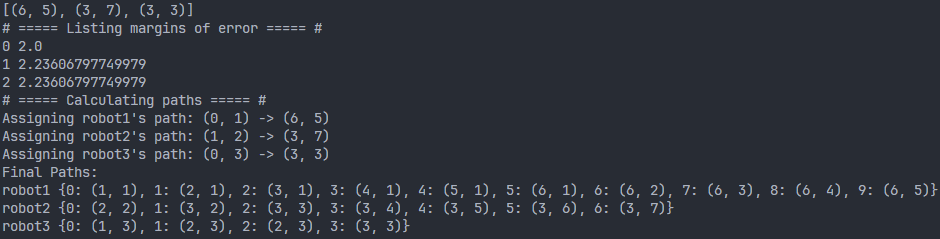
\includegraphics[width=1\linewidth]{assets/images/formation/console_output.png}
    \caption{Console Output}
    \label{fig:formation_console_output}
\end{figure}

\paragraph*{}
Nevertheless, this path planning algorithm still contains a glaring flaw. It currently does not consider obstacles in the environment. This can be seen as a room for improvement; or perhaps other modules can assist in offsetting this current drawback.

\begin{figure}
    \centering
    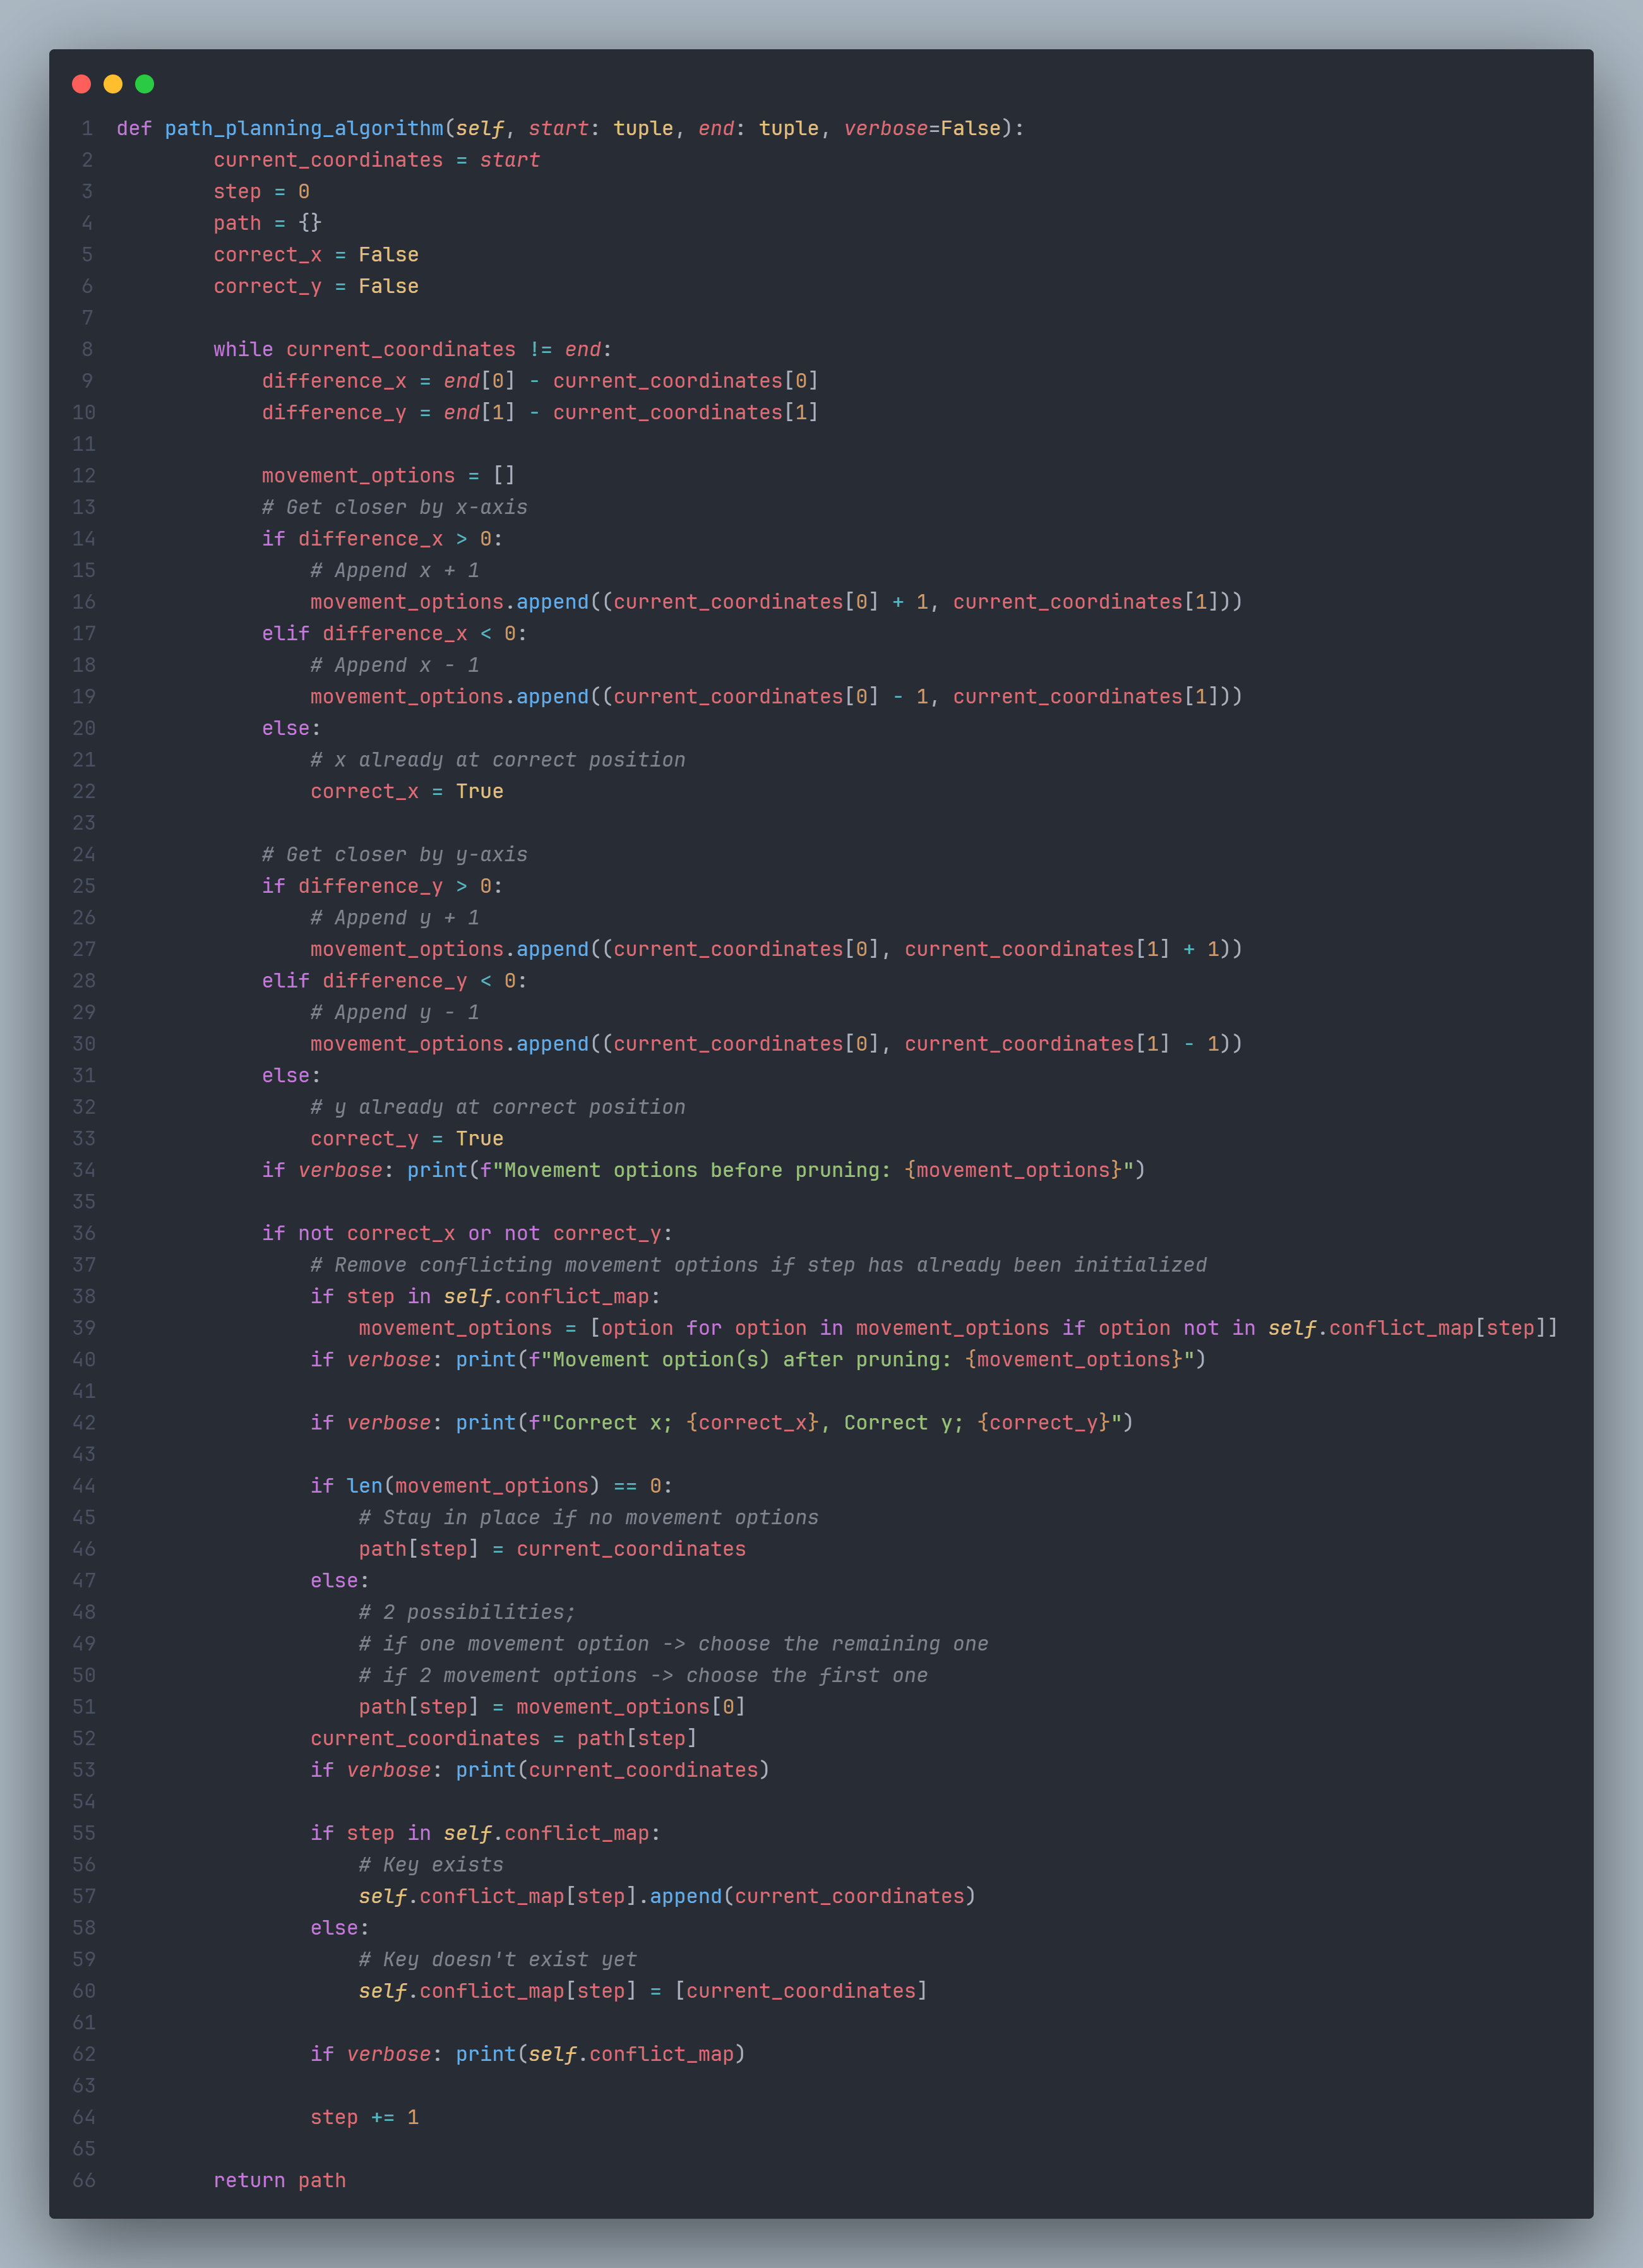
\includegraphics[width=1\linewidth]{assets/images/formation/path_planning_algorithm.png}
    \caption{Path Planning Algorithm}
    \label{fig:formation_path_planning_algorithm}
\end{figure}
